\documentclass[11pt]{article}
\pagestyle{empty}
\usepackage{amsmath,amssymb,amsfonts,setspace,float,enumerate}
\usepackage{graphicx,mathtools}
\usepackage[margin=1in]{geometry}
\usepackage{hyperref}
\usepackage{xcolor}
\usepackage{subcaption}
\hypersetup{
	colorlinks=true,
    linkbordercolor={1 1 1},
    linkcolor = red
}
\parindent 0px
\pagenumbering{gobble}
\singlespacing

\title{Braess's Paradox Write Up}
\author{David Ye}
\date{\today}

\begin{document}
\maketitle
\section{Results}
The best lane configuration obtained from simulated annealing is:
\begin{align*}
\begin{bmatrix}
0 & 0 & 5 & 0\\
0 & 0 & 5 &5\\
5 & 5 & 0 & 0\\
0 & 5 & 0 & 0
\end{bmatrix}
\end{align*}
The average energy of this lane configuration is 0.00623. A snapshot of the simulation is displayed in figure \ref{fig:snapshot}. To identify the four location shown in figure figure \ref{fig:snapshot}, lets let A represent the top left location, B represent the top middle location, C represent the bottom middle location, and D represent the bottom right location.
\begin{figure}[H]
	\centering
	\includegraphics[width=10cm]{Snapshot.png}
	\caption{\label{fig:snapshot} A snapshot of the best lane configuration}
\end{figure}

The lane configuration returned by simulated annealing is quite surprising since it does not remove the lanes between locations B and C as mentioned in the handout. Rather, the lanes between locations B and C were set to the max possible lanes and the lanes between locations A and B, and the lanes between location C and D were completely removed. Table \ref{table:compare} compares the performance of the best lane configuration returned by SA and the lane configuration suggested in the handout. We see the best lane configuration returned from SA has an average energy of 0.00623 while the lane configuration mentioned in the handout has an average energy of 0.107. Thus, the former lane configuration has $94\%$ less energy than the latter, a significant improvement.

\begin{table}[H]
\centering
\begin{tabular}{|l|l|l|}
\hline
Lane Configuration & Average Energy & Lane Configuration Matrix\\ \hline
From SA (best)& 0.00623 &  [[0, 0, 5, 0], [0, 0, 5, 5], [5, 5, 0, 0], [0, 5, 0, 0]]\\ \hline
From Handout &  0.107 & [[0, 2, 5, 0], [2, 0, 0, 5], [5, 0, 0, 2], [0, 5, 2, 0]]\\ \hline
\end{tabular}
\caption{\label{table:compare} Table comparing average energy of best lane configuration obtained from SA and lane configuration mentioned in handout.}
\end{table}

In figure \ref{fig:snap} we see a side by side snapshot of both lane configurations. The handout lane configuration (shown on the right of \ref{fig:snap}) has three directions of travel where the number of cars on the roads are equal or greater than the road capacity. Meanwhile, the lane configuration returned from SA (shown on the left) has no directions of travel where the number of cars on the roads are equal or greater than the road capacity meaning less traffic.

\begin{figure}[H]%
    \centering
    \subfloat[\centering Best Lane Configuration from SA]{{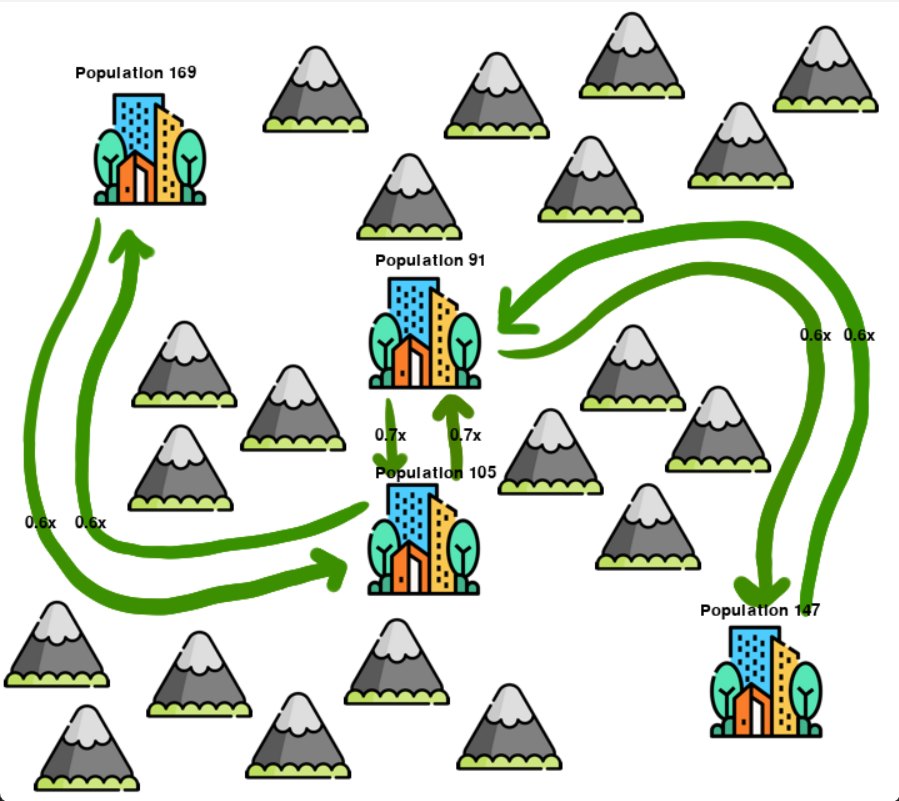
\includegraphics[width=7cm]{snapshot.png} }}%
    \qquad
    \subfloat[\centering Lane Configuration from Handout]{{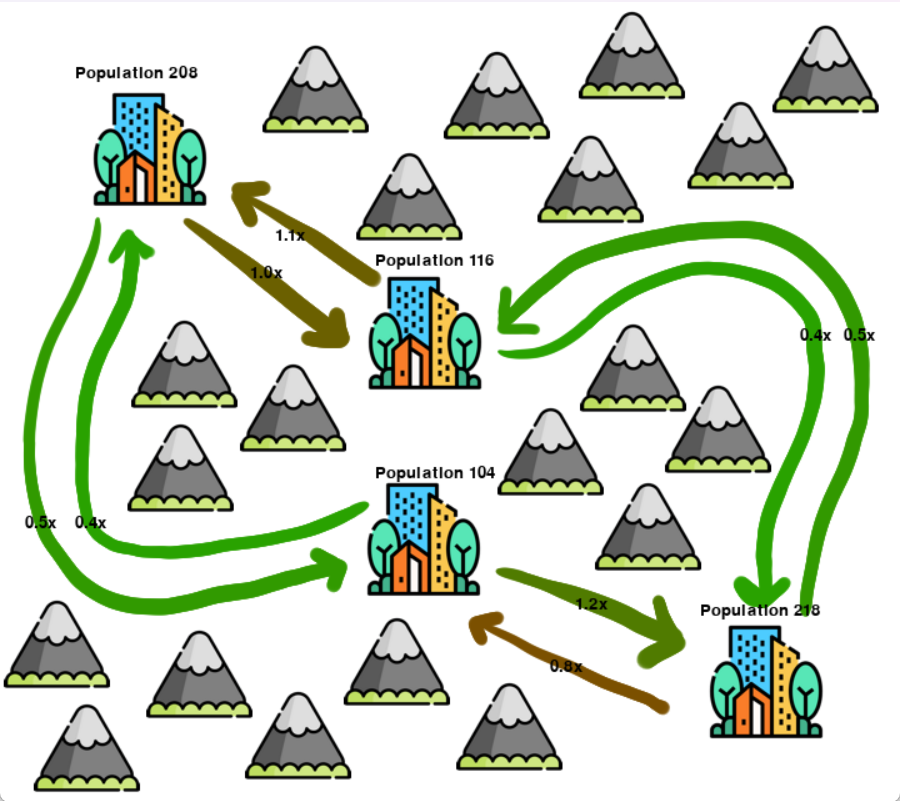
\includegraphics[width=7cm]{Handout.png} }}%
    \qquad
    \caption{Snapshots of different lane configurations}%
    \label{fig:snap}%
\end{figure}

I am very surprised that the best lane configuration uses only 30 of the 38 available lanes. This is over $20\%$ less than the maximum number of lanes allowed! Yet, this lane configuration is superior to all other lane configurations I've seen. 

In the context of Braess's paradox, this configuration does make sense. We can observe by including directions of travel limited to only two lanes, the result is moderate amounts of traffic as seen between locations A and B, and locations C and D as seen in figure \ref{fig:snap} with the snapshot on the right. However, by removing all directions of travel that are limited to two lanes, we essentially eliminate traffic altogether. This is because five lanes have more than enough capacity to support even the highest traffic volumes between locations B and C as seen in figure \ref{fig:snap} with the snapshot on the left. The pros of the lane configuration returned by SA is there will be essentially no traffic whatsoever. The cons is cars will need to travel much further to get to their destinations (especially to and from locations A and D).
\section{Modifications}

I tried out five different approaches for choosing neighboring lane matrices. Below is a brief description of each approach:
\begin{enumerate}
	\item Random: Choose a random element in the lane configuration matrix and set the number of lanes to a random integer between 0 and the max number of roads allowed.
	\item Symmetric Random: Choose a random element in the lane configuration matrix. Then set the number of lanes to a random integer between 0 and the max number of roads allowed for both the random element selected as well as the reverse direction of the random element selected (change number of lanes going to and from location A and B to same random integer).
	\item Incremental: Randomly select an element in the lane configuration matrix. Choose a random number between 0 and 1. If the random number is less than or equal to 0.5, reduce the number of lanes by one. If the random number is greater than 0.5, increase the number of lanes by one. Note: conditions are set in place to ensure the number of lanes do not decrease below zero or increase over the max number of lanes allowed.
	\item All or Nothing: Randomly select an element in the lane configuration matrix. Choose a random number between 0 and 1. If the random number is less than 0.5, set the number of lanes to zero. If the random number is greater or equal to 0.5, set the number of lanes to the max number of roads allowed.
	\item Symmetric All or Nothing: Randomly select an element in the lane configuration matrix. Choose a random number between 0 and 1. If the random number is less than 0.5, set the number of lanes to zero for both the selected element as well as the opposite direction of the selected element (i.e. going from A to B, going from B to A). If the random number is greater or equal to 0.5, set the number of lanes to the max number of roads allowed for both the selected element as well as the opposite direction of the selected element.
\end{enumerate}
A summary of the performance of each approach is listed in table \ref{table:neighbor}.
\begin{table}[H]
\centering
\begin{tabular}{|l|l|l|}
\hline
Neighbor Selection Approach & Average Energy & Lane Configuration Matrix\\ \hline
Random& 0.106 &   [[0, 2, 5, 0], [2, 0, 0, 5], [5, 0, 0, 2], [0, 3, 2, 0]]\\ \hline
Symmetric Random &   0.101 &  [[0, 2, 5, 0], [2, 0, 0, 2], [5, 0, 0, 2], [0, 2, 2, 0]]\\ \hline
Incremental &  0.215 & [[0, 2, 5, 0], [2, 0, 4, 5], [4, 4, 0, 2], [0, 4, 2, 0]]\\ \hline
All or Nothing &  0.107 &  [[0, 2, 5, 0], [2, 0, 0, 5], [5, 0, 0, 2], [0, 5, 2, 0]]\\ \hline
Symmetric All or Nothing &   0.00623 &  [[0, 0, 5, 0], [0, 0, 5, 5], [5, 5, 0, 0], [0, 5, 0, 0]]\\ \hline
\end{tabular}
\caption{\label{table:neighbor} Table comparing average energy of the best matrix obtained from various implementations of simulated annealing.}
\end{table}
A visualization of the lane configuration obtained from each approach is displayed in figure \ref{fig:neighbor}.
\begin{figure}[H]%
    \centering
    \subfloat[\centering Random]{{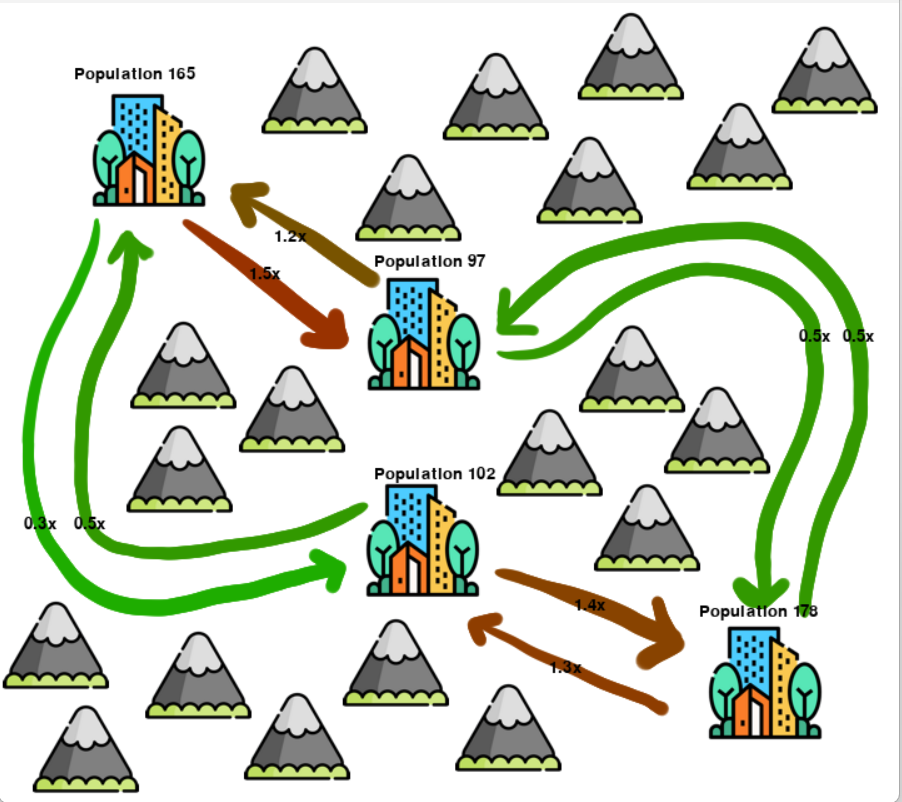
\includegraphics[width=7cm]{random.png} }}%
    \qquad
    \subfloat[\centering Symmetric Random]{{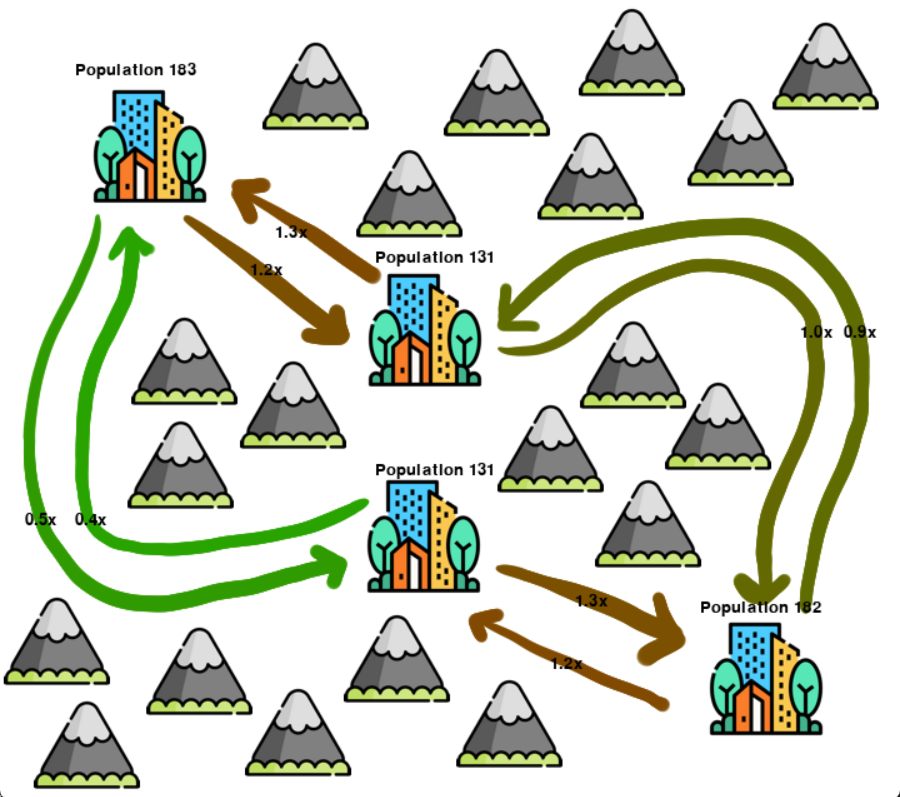
\includegraphics[width=7cm]{symmetricRandom.png} }}%
    \qquad
    \subfloat[\centering Incremental]{{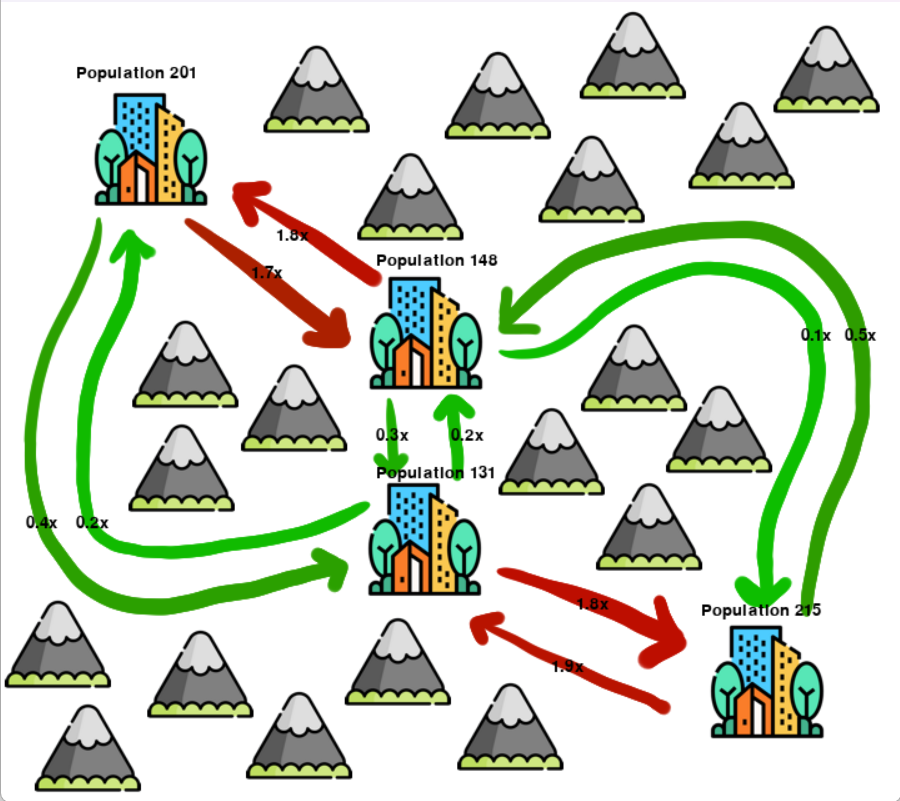
\includegraphics[width=7cm]{Incremental.png} }}%
    \qquad
    \subfloat[\centering All or Nothing]
{{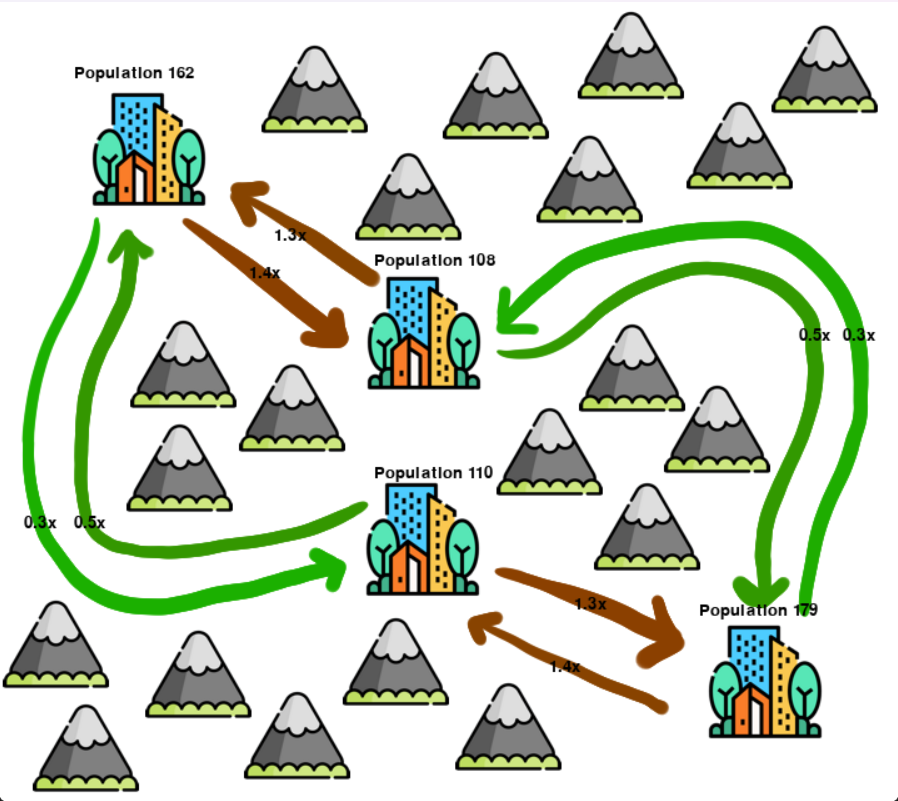
\includegraphics[width=7cm]{AllOrNothing.png} }}%
    \qquad
    \subfloat[\centering Symmetric All or Nothing]
{{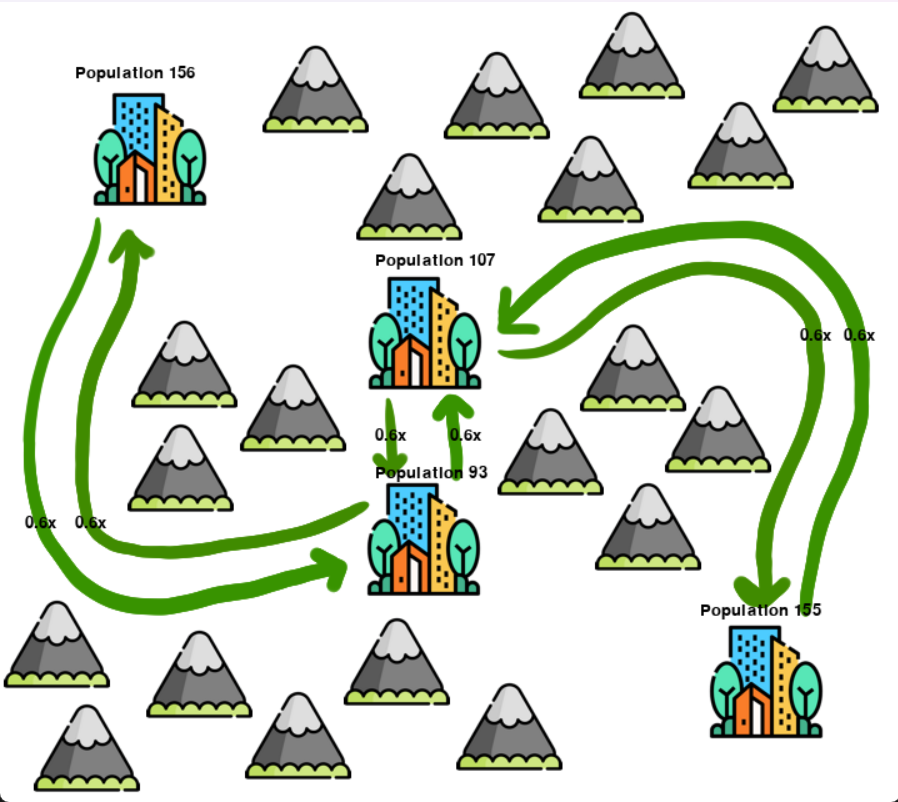
\includegraphics[width=7cm]{SymAllOrNothing.png} }}%
    \caption{Snapshots of lane configurations obtained from various implementations of simulated annealing}%
    \label{fig:neighbor}%
\end{figure}
From the above table and snapshots, we see the symmetric all or nothing neighbor selection approach returned the best lane configuration and the lowest energy (0.00623). This lane configuration has $94\%$ less energy than the next best lane configuration. The symmetric approach works well people are leaving and arriving at locations at a similar rate. This may be because the population of pairs of locations are symmetric, and also people randomly selecting new destination. As a result, have the same number of lanes going to and from a location is beneficial. The symmetric all or nothing approach works well because it does not get stuck in local minimums like the other approaches often do. The idea behind the all or nothing is its either better to leave two locations disconnected, or its better to utilize the max number of lanes possible; there is no in-between. Because of the binary-like options, there are a lot fewer options to choose from. This makes finding the global minimum quite a bit easier and faster.

I also made modifications to the number of lanes as well as the departure rate in an effort to replicate the suggested lane configuration in the handout. My idea was to increase the departure rate until congestion developed between locations B and C, or to decrease the number of lanes between locations B and C until congestion develops. At that point, it would likely be better to remove the lanes connecting location B and C and keep the lanes connecting A to B and C to D.

The departure rates I simulated includes: 25, 100, 200, 300, 400, 500, 700, and 1000. For each departure rate, I ran 50 iterations of simulated annealing. The results are shown in table \ref{table:departResults} where average energy represents the average energy of the best found lane configuration (averaged over 5 iterations). Snapshots of the best lane configurations obtained for various departure rates are shown in figure \ref{fig:departFig}.

At a departure rate of 25, the energy was smallest (least traffic). The energy increased as departure rate increased to 100. Surprisingly, between departure rates 200 to 1000, the energy remained relatively the same. There was not enough cars on the road to cause congestion, even with a departure rate of 1000. As a result, the best lane configuration continued to keep the lanes between locations B and C.

\begin{table}[H]
\centering
\begin{tabular}{|l|l|l|}
\hline
Departure Rate & Average Energy & Lane Configuration\\ \hline
25 & 0.000231 &  [[0, 0, 5, 0], [0, 0, 5, 5], [5, 5, 0, 0], [0, 5, 0, 0]]\\ \hline
100 & 0.00620 & [[0, 0, 5, 0], [0, 0, 5, 5], [5, 5, 0, 0], [0, 5, 0, 0]]\\ \hline
200 &  0.00805 & [[0, 0, 5, 0], [0, 0, 5, 5], [5, 5, 0, 0], [0, 5, 0, 0]]\\ \hline
300 &  0.00855 &  [[0, 0, 5, 0], [0, 0, 5, 5], [5, 5, 0, 0], [0, 5, 0, 0]]\\ \hline
400 & 0.00874 &  [[0, 0, 5, 0], [0, 0, 5, 5], [5, 5, 0, 0], [0, 5, 0, 0]]\\ \hline
500 &  0.00888 &  [[0, 0, 5, 0], [0, 0, 5, 5], [5, 5, 0, 0], [0, 5, 0, 0]]\\ \hline
700 & 0.00890  & [[0, 0, 5, 0], [0, 0, 5, 5], [5, 5, 0, 0], [0, 5, 0, 0]] \\ \hline
1000 &  0.00905&  [[0, 0, 5, 0], [0, 0, 5, 5], [5, 5, 0, 0], [0, 5, 0, 0]] \\ \hline
\end{tabular}
\caption{\label{table:departResults} Table comparing average energy of best lane configurations obtained from SA for various departure rates}
\end{table}


\begin{figure}[H]%
    \centering
    \subfloat[\centering Departure Rate: 25]{{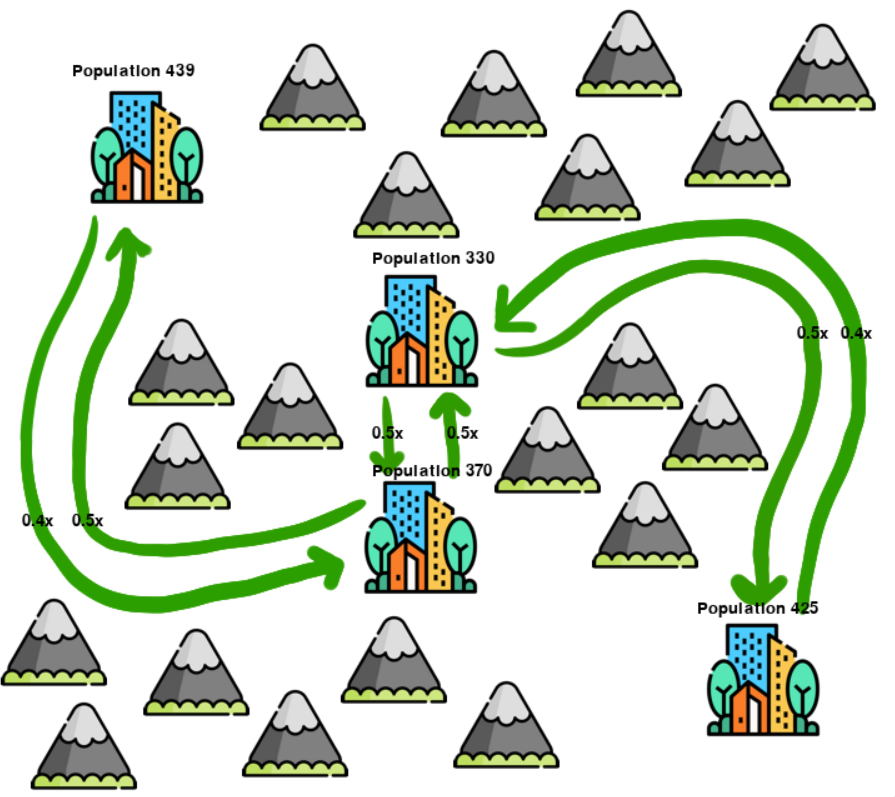
\includegraphics[width=5cm]{25.png} }}%
    \qquad
    \subfloat[\centering Departure Rate: 100]{{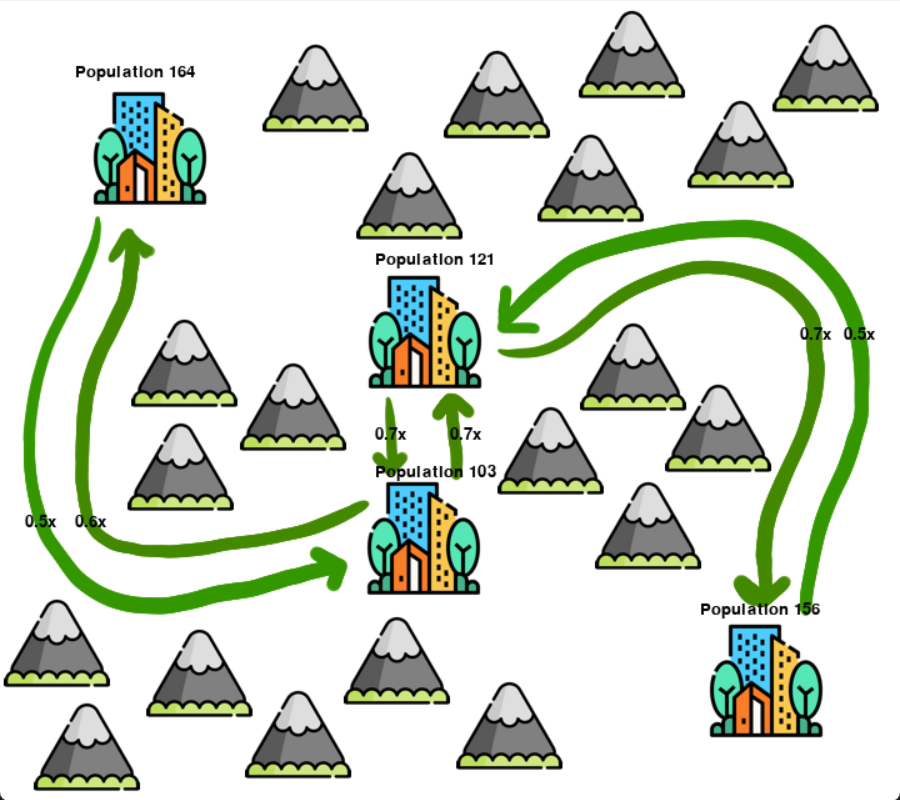
\includegraphics[width=5cm]{100.png} }}%
    \qquad
    \subfloat[\centering Departure Rate: 200]{{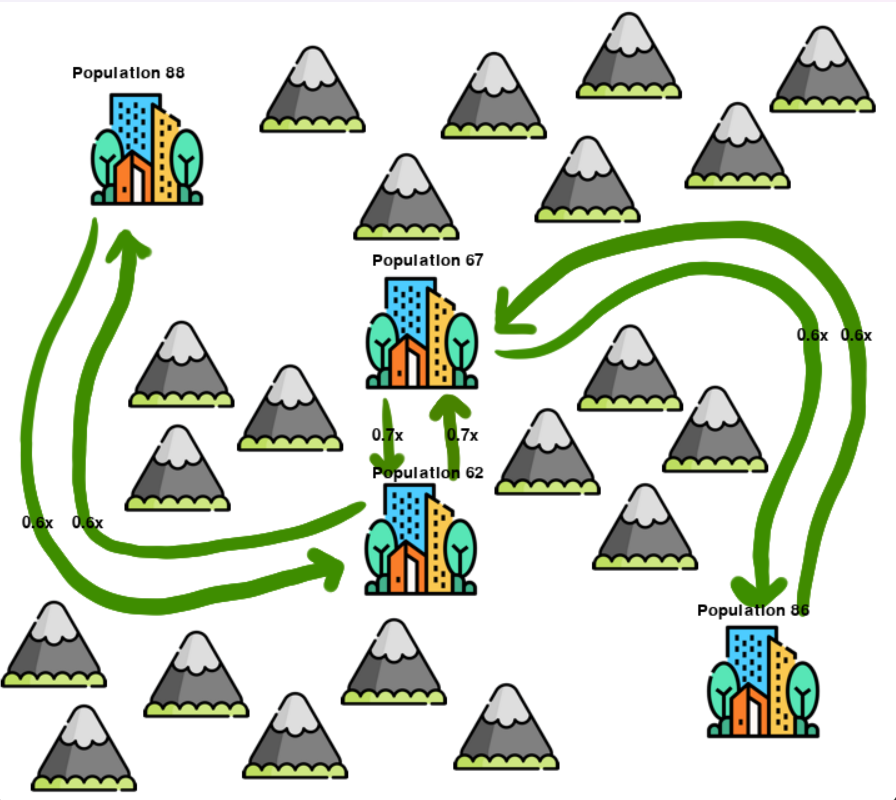
\includegraphics[width=5cm]{200.png} }}%
    \qquad
    \subfloat[\centering Departure Rate: 300]
{{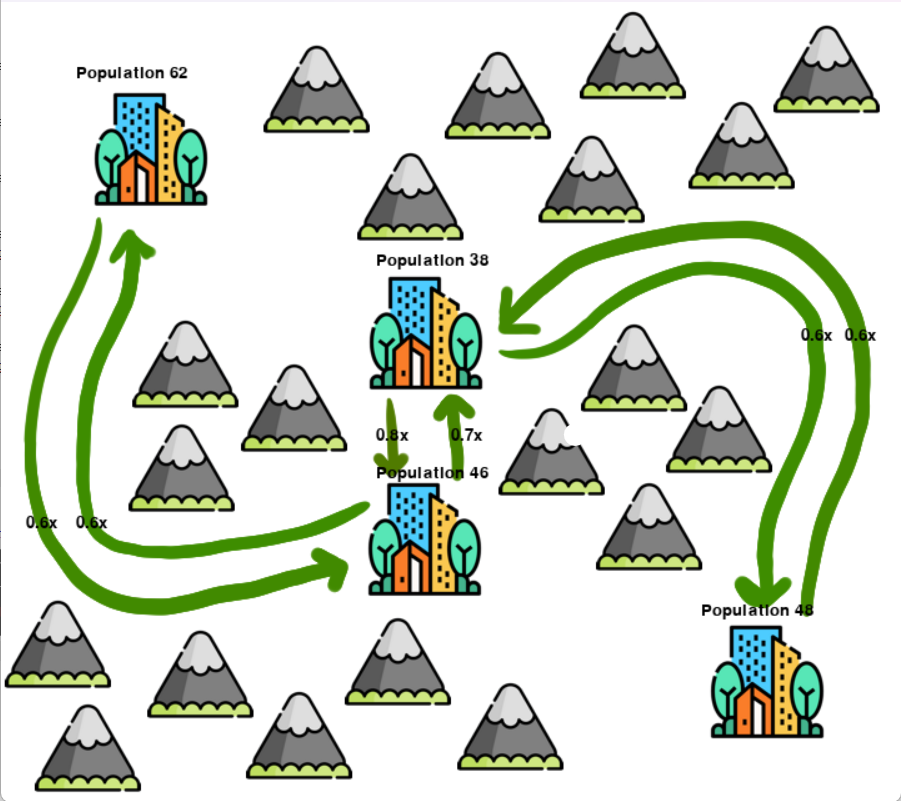
\includegraphics[width=5cm]{300.png} }}%
    \qquad
    \subfloat[\centering Departure Rate: 400]
{{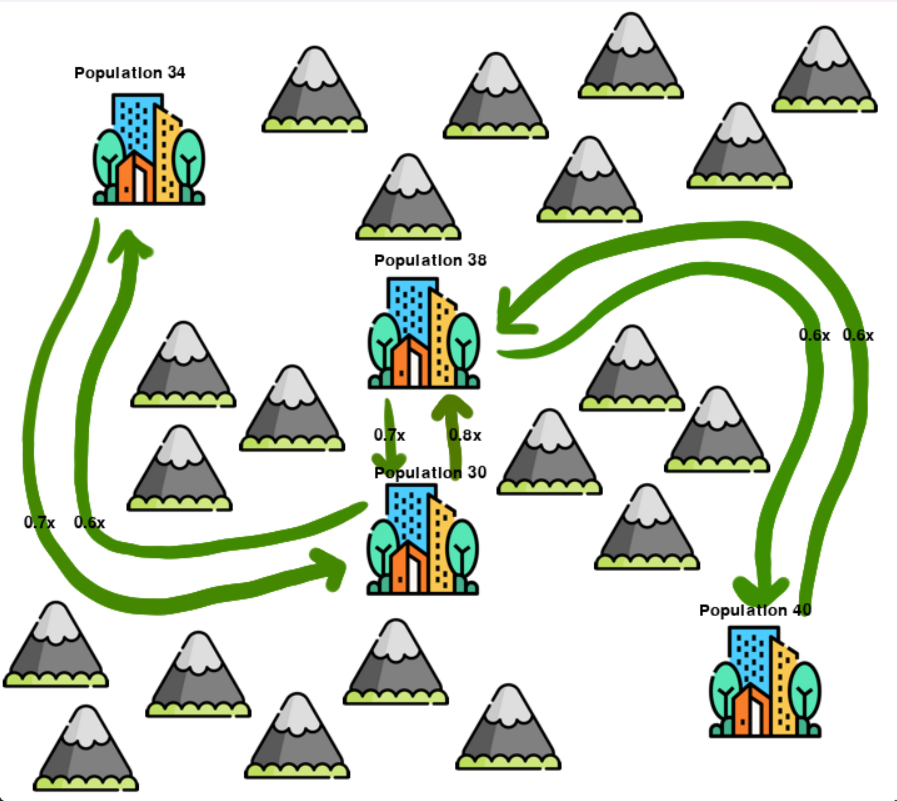
\includegraphics[width=5cm]{400.png} }}%
    \qquad
    \subfloat[\centering Departure Rate: 500]  
{{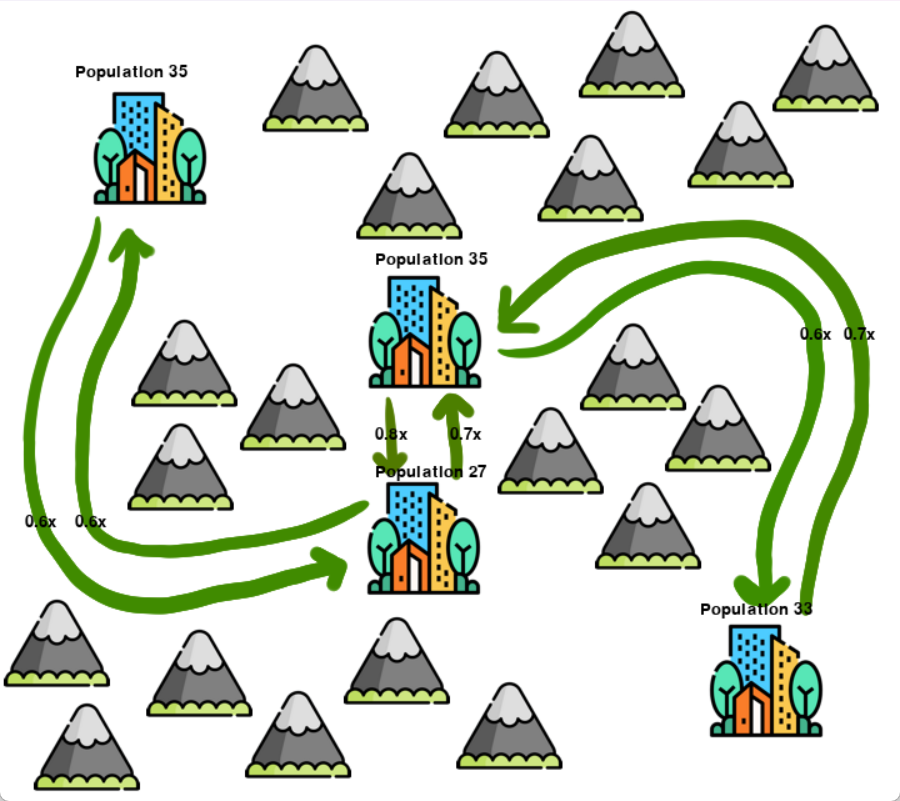
\includegraphics[width=5cm]{500.png} }}%
	\qquad
    \subfloat[\centering Departure Rate: 700]  
{{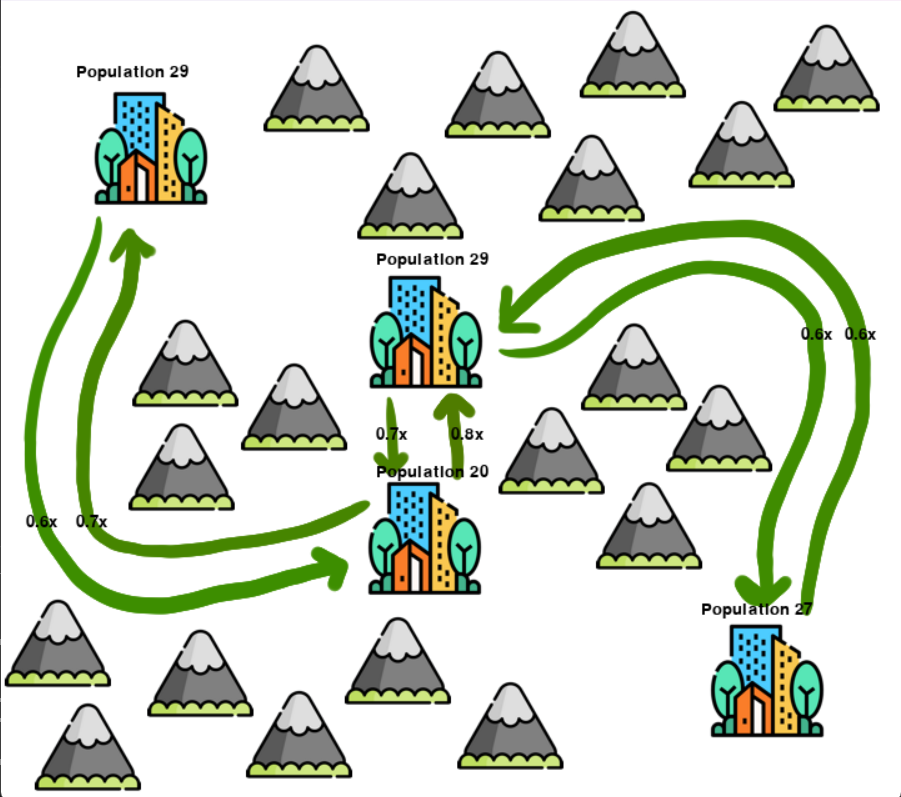
\includegraphics[width=5cm]{700.png} }}%
	\qquad
    \subfloat[\centering Departure Rate: 1000]  
{{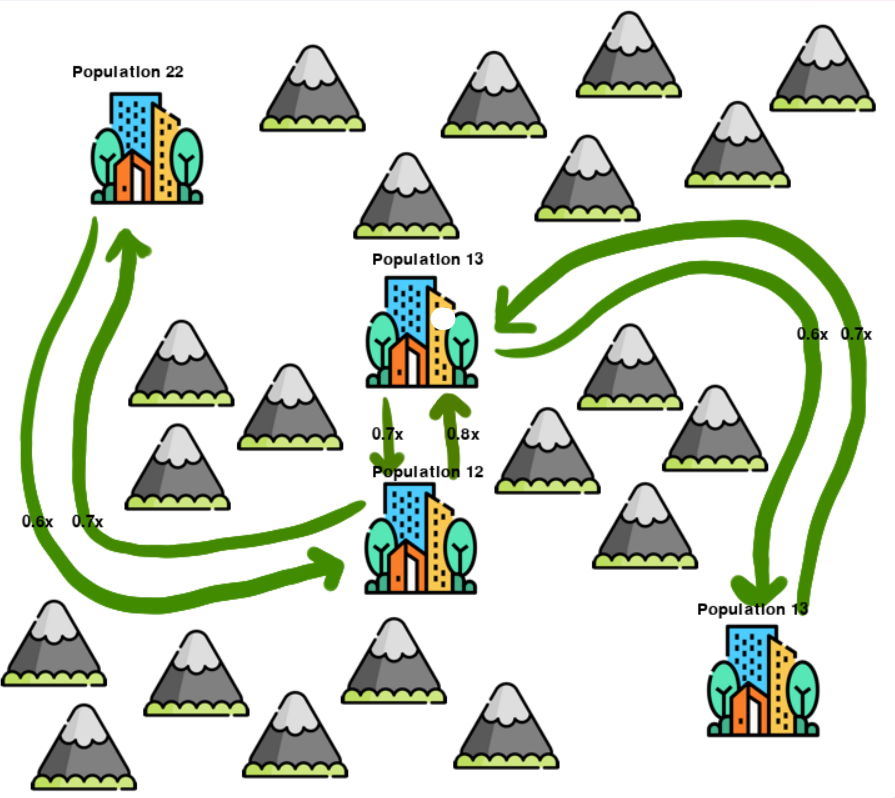
\includegraphics[width=5cm]{1000.png} }}%
    \caption{Snapshots of simulations for various departure rates}%
    \label{fig:departFig}%
\end{figure}

Last but not least, when I reduced the max number of lanes between location B and C to 1, the best lane configuration I obtained was identical to the one mentioned in the handout (lane matrix: [[0, 2, 5, 0], [2, 0, 0, 5], [5, 0, 0, 2], [0, 5, 2, 0]], energy: 0.107). With only one lane from B to C and one lane from C to B, there was too much traffic. To reduce the traffic, all roads between B and C were cut, and roads between locations A and B, and C and D were added back in. A snapshot of the simulation is shown in figure \ref{fig:maxLim}.

\begin{figure}[H]%
    \centering
    \subfloat[\centering Departure Rate: 1000]  
{{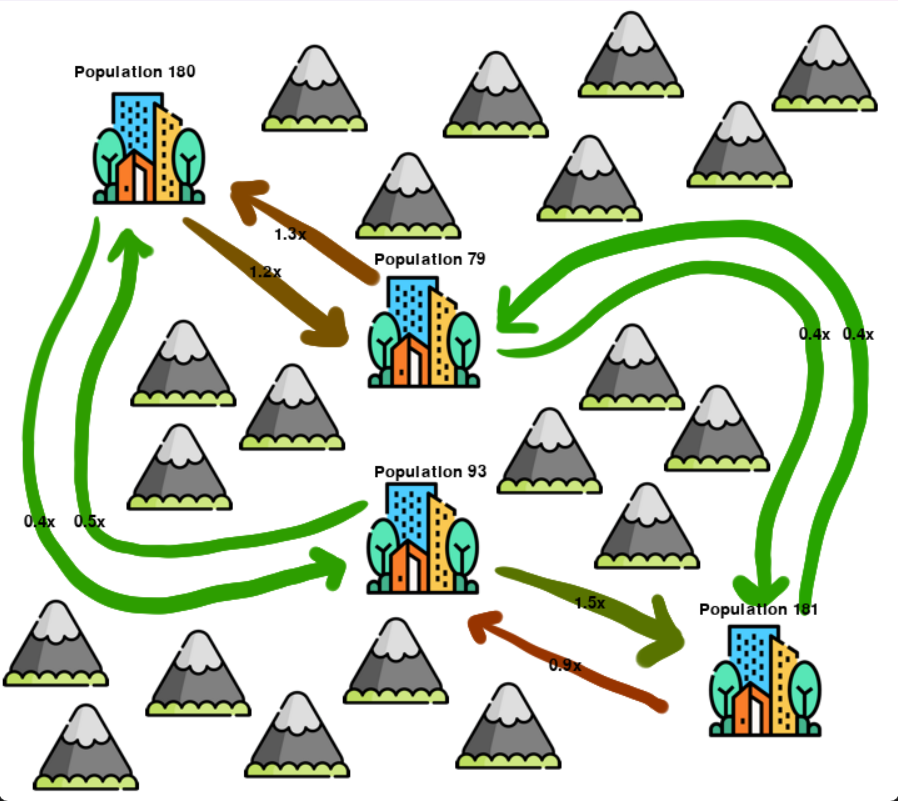
\includegraphics[width=8cm]{maxLim.png} }}%
    \caption{Snapshots of simulations for various departure rates}%
    \label{fig:maxLim}%
\end{figure}


\section{Simplifications and Limitations}
There are many simplification that goes into our traffic modeling. For example, our model neglects traffic lights, pedestrians (i.e. crosswalks), and any mode of transportation other than cars. Our model also assumes cars travel at a constant 60 mph on all roads. In real life, this is far from the case. For example, on local roads speed limits will be much lower than on freeways. Another simplification is our model has a constant departure rate. In reality, traffic on weekends is different from traffic on weekdays. And traffic during rush hour is different from traffic during noon or midnight.

One limitation of our simulation is the destinations chosen for people at home are random. In reality, there are cities and suburbs. People are likely to have preferences on where they want to go. Also, people are habitual drivers. There are likely strong patterns that exist throughout the temporal and spatial field, that cannot be spotted using our simulation.

While researching other methods of modeling traffic, I concluded our model likely falls under mesoscopic simulation. Mesoscopic simulations combine properties of both microscopic simulations (individual people waiting and cars leaving at random times to random destinations) as well as macroscopic simulations (constant rate of departure, constant car following distance, constant car speed). 

Besides Monte Carlo methods, other ways of simulating traffic include cellular automata models, car-following models, discrete event and continuous-time simulations, and numerical ODE/PDE methods.


\end{document}